\chapter[Referencial Teórico]{Referencial Teórico}
\label{sec:referencial}

\section{Bancos de dados relacionais}

Os bancos de dados relacionais constituem um paradigma amplamente adotado no gerenciamento de dados, fundamentado na utilização de tabelas para representar tanto os dados em si quanto as relações entre eles. O modelo relacional é o mais prevalente entre os modelos de dados, sustentando a maioria dos sistemas de gerenciamento de banco de dados atuais, devido à sua eficiência e flexibilidade na representação de dados \cite{silberschatz2011database}.

As tabelas em um banco de dados relacional são compostas por linhas e colunas, onde cada linha representa um registro e cada coluna corresponde a um campo de dado específico. A inter-relação entre as tabelas é realizada por meio de chaves primárias e chaves estrangeiras, permitindo a integração e o acesso eficiente aos dados armazenados \cite{silberschatz2011database}.

Na Figura \ref{fig:exemplo}, pode-se observar um exemplo de tabela que representa um banco de dados com informações de funcionários. A tabela apresenta dados organizados em colunas que indicam o identificador único (\textit{id}) de cada funcionário, o nome, o departamento ao qual pertencem e seus respectivos salários. Esse exemplo ilustra uma estrutura típica utilizada bancos de dados relacionais.

\begin{figure}[H]
    \centering
    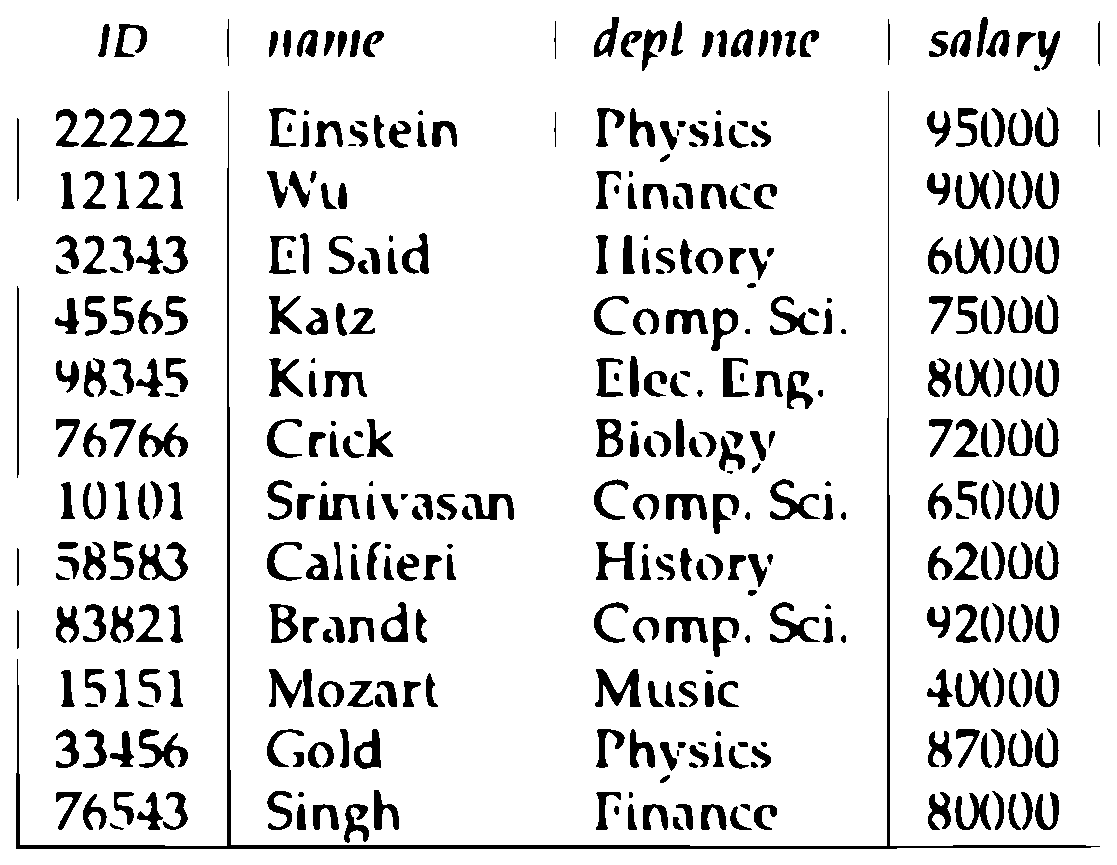
\includegraphics[width=0.5\textwidth]{figuras/tabela_silbershatz.eps}
    \caption{Tabela em um banco de dados relacional}
    Fonte: \cite{silberschatz2011database}
    \label{fig:exemplo}
\end{figure}

\subsection{SQL}

A Linguagem de Consulta Estruturada (SQL), desenvolvida inicialmente pela IBM nos anos 1970 sob o nome Sequel, consolidou-se como o padrão para a manipulação de bancos de dados relacionais. SQL se destaca por sua natureza não procedural, permitindo que consultas sejam realizadas sobre uma ou várias tabelas. Além de sua função primária de consulta, SQL é capaz de definir a estrutura dos dados, modificar informações armazenadas e estabelecer restrições de segurança. A linguagem é amplamente suportada por diversos produtos, solidificando sua posição como o idioma universal dos bancos de dados relacionais \cite{silberschatz2011database}.

A linguagem SQL mantém-se como uma das tecnologias mais significativas no campo do desenvolvimento. SQL é utilizada por 51\% de todos os respondentes, destacando-se como uma das quatro principais tecnologias, ao lado de JavaScript, HTML/CSS e Python. Essa ampla adoção indica a relevância de SQL na manipulação e gestão de dados, essencial para aplicações que requerem o armazenamento e a recuperação eficiente de informações em bases de dados relacionais \cite{StackOverflow2024}.

Além disso, a importância de SQL é ainda mais pronunciada entre desenvolvedores profissionais, conforme a mesma pesquisa, onde a sua utilização atinge 54.1\%, posicionando-a logo após JavaScript. Este dado ressalta a aplicação crítica de SQL em ambientes corporativos, onde a eficiência, a integridade e a segurança no gerenciamento de dados são prioritárias. A \textit{expertise} em SQL possibilita aos desenvolvedores a realização de consultas complexas, a otimização de desempenho e a garantia de integridade dos dados, habilidades indispensáveis na análise de grandes volumes de informações e essenciais para suportar as demandas de negócios modernos. Portanto, a proficiência em SQL continua a ser uma competência essencial no arsenal de habilidades de qualquer profissional de tecnologia da informação \cite{StackOverflow2024}.


\subsubsection{Linguagem de Definição de Dados (DDL)}

A Linguagem de Definição de Dados (DDL) em SQL é uma ferramenta na especificação do esquema de um banco de dados relacional, permitindo a definição de diversas características essenciais para cada relação. Por meio da DDL, é possível delinear a estrutura do banco de dados, especificando o esquema de cada relação, os tipos de dados associados a cada atributo e impondo restrições de integridade para assegurar a consistência dos dados, como a definição de chaves primárias. A execução de comandos DDL gera metadados, que são armazenados no dicionário de dados do sistema, um repositório acessado apenas pelo sistema de banco de dados. Este dicionário é consultado durante operações de leitura ou modificação de dados, garantindo que as atualizações atendam às restrições estabelecidas, preservando a integridade e a eficiência do sistema.\cite{silberschatz2011database}

A Linguagem de Definição de Dados (DDL) abrange comandos que possibilitam a criação, alteração e exclusão de esquemas de banco de dados, tabelas, índices e outros objetos. Exemplos de comandos DDL incluem \textit{CREATE}, \textit{ALTER}, \textit{DROP}, \textit{TRUNCATE} e \textit{RENAME}. Esses comandos serão melhor exemplificados a seguir:

\subsubsubsection{CREATE}

O comando \textit{CREATE}, na linguagem SQL (\textit{Structured Query Language}), que faz parte da Linguagem de Definição de Dados (DDL), tem como função principal a criação de novos objetos no banco de dados. Entre os comandos disponíveis, o \textit{CREATE TABLE} é frequentemente empregado, sendo responsável pela definição de tabelas que armazenarão os dados. A configuração de uma tabela requer a especificação de colunas, tipos de dados e restrições, como chaves primárias e estrangeiras\cite{silberschatz2011database}.

\begin{figure}[H]
    \centering
    \begin{lstlisting}
    CREATE TABLE nome_da_tabela (
    coluna1 tipo_de_dado,
    coluna2 tipo_de_dado,
    ...
    colunaN tipo_de_dado
    );
        \end{lstlisting}
    \caption{Comando SQL de criação}
    Fonte: Autor
    \label{lst:sql_create}
\end{figure}


Na figura \ref{fig:create_table}, O comando SQL apresentado cria a tabela PROJECT, que armazena informações sobre projetos, incluindo nome, número, localização e departamento associado. A coluna Pname armazena o nome do projeto, limitado a 15 caracteres, obrigatório e com restrição de unicidade. O Pnumber, que é a chave primária da tabela, garante que cada projeto tenha um número exclusivo. A coluna Plocation, que também aceita até 15 caracteres, é opcional e pode ser nula. Por último, a coluna Dnum armazena o número do departamento responsável, sendo obrigatória e definida como chave estrangeira, relacionando-se com a coluna Dnumber da tabela DEPARTMENT. Essa estrutura exemplifica a criação de uma tabela relacional com regras de integridade e relacionamento entre tabelas no banco de dados.

\begin{figure}[H]
    \centering
    
\includegraphics[width=0.8\textwidth]{figuras/create_table_elmasi.eps}
    \caption{Comando SQL - Criação de uma tabela}
    Fonte: \cite{elmasri2011fundamentals}
    \label{fig:create_table}
\end{figure}


\subsubsubsection{ALTER}

O comando \textit{ALTER TABLE} é um recurso utilizado na manipulação de esquemas de bancos de dados, permitindo a modificação de relações existentes. Por meio deste comando, é possível adicionar novos atributos a uma tabela, os quais inicialmente são atribuídos como nulos para todas as tuplas, ou eliminar atributos já existentes, sendo que a possibilidade de exclusão pode variar entre diferentes sistemas de gerenciamento de banco de dados. A utilização do comando \textit{ALTER TABLE} é relevante para a manutenção da integridade e evolução dos dados em um banco de dados ao longo do tempo \cite{silberschatz2011database}.


\begin{figure}[H]
    \centering
    \begin{lstlisting}
    ALTER TABLE nome_da_tabela
    ADD coluna_nova tipo_de_dado;
    \end{lstlisting}
    \caption{Comando SQL - criação nova coluna usando \textit{ALTER}}
    Fonte: Autor
    \label{lst:sql_alter}
\end{figure}


O comando ALTER é empregado para realizar  operações como:  adição, modificação ou exclusão de colunas em uma tabela, ajustes em restrições (como chaves primárias e estrangeiras), e modificações de tipos de dados \cite{silberschatz2011database}. Por exemplo, na figura \ref{fig:alter_table}, a adição de uma nova coluna \textit{Job} a tabela \textit{EMPLOYEE} pode ser realizada através do comando \textit{ALTER TABLE}. Esta flexibilidade é crucial para a manutenção e evolução de sistemas de banco de dados, permitindo adaptações às necessidades dinâmicas das aplicações que os utilizam.

\begin{figure}[H]
    \centering
    
\includegraphics[width=0.7\textwidth]{figuras/alter_table_elmasi.eps}
    \caption{Exemplo SQL - \textit{ALTER TABLE}}
    Fonte: \cite{elmasri2011fundamentals}
    \label{fig:alter_table}
\end{figure}

\subsubsubsection{DROP}

O comando \textit{DROP} em SQL desempenha um papel crucial na gestão de bancos de dados, permitindo a remoção de relações, tipos, esquemas e índices de forma permanente. Especificamente, o comando \textit{DROP TABLE} é utilizado para excluir uma tabela e todas as suas informações associadas, representando uma ação drástica que não pode ser revertida \cite{silberschatz2011database}.

\begin{figure}[H]
    \centering
    \begin{lstlisting}
    DROP TABLE nome_da_tabela;
    \end{lstlisting}
    \caption{Comando SQL de criação nova coluna }
    Fonte: Autor
    \label{lst:sql_drop}
\end{figure}

\subsubsubsection{TRUNCATE}

O comando \textit{TRUNCATE TABLE} na linguagem SQL é um procedimento que permite a remoção completa dos dados contidos em uma tabela, sendo classificado como uma instrução de Linguagem de Definição de Dados (DDL). A operação de truncamento é realizada de maneira eficiente, uma vez que envolve a exclusão e recriação da tabela, o que resulta em um desempenho superior, especialmente em tabelas grandes. No entanto, o uso do \textit{TRUNCATE} é restrito em situações onde existem restrições de chave estrangeira que referenciam a tabela alvo.\cite{mySQL2025}

\begin{figure}[H]
    \centering
    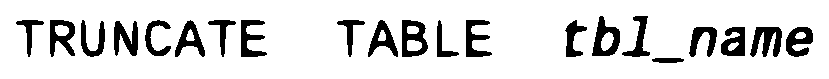
\includegraphics[width=0.4\textwidth]{figuras/truncate_mysql.eps}
    \caption{Trucante MYSQL}
    Fonte: Autor
    \label{fig:truncate}
\end{figure}


\subsubsubsection{RENAME}

O comando \textit{RENAME TABLE} é uma instrução no gerenciamento de bancos de dados que, permite a renomeação de uma ou mais tabelas de forma eficiente e em uma única operação. Diferentemente do comando \textit{ALTER TABLE}, que renomeia apenas uma tabela, o \textit{RENAME TABLE} possibilita a renomeação simultânea de várias tabelas, considerando a ordem em que são especificadas na instrução. 

\begin{figure}[H]
    \centering
    \begin{lstlisting}
    RENAME TABLE nome_da_tabela_antiga TO nome_da_tabela_nova;
    \end{lstlisting}
    \caption{Comando SQL de renomeação}
    Fonte: Autor
    \label{lst:sql_rename}
\end{figure}

\subsubsection{Linguagem de Manipulação de Dados (DML)}

A DML é utilizada para realizar operações de inserção, atualização e exclusão de dados armazenados nas tabelas. A DML é fundamental para a manutenção e modificação dos dados de maneira dinâmica. Os comandos \textit{INSERT}, \textit{UPDATE} e \textit{DELETE} são exemplos típicos de operações DML \cite{silberschatz2011database}.

\subsubsubsection{INSERT}

O comando \textit{INSERT}, integrante da linguagem de manipulação de dados (DML) do SQL, é fundamental para a inclusão de novas tuplas em uma relação dentro de um banco de dados. Sua aplicação pode ocorrer de duas maneiras: através da especificação direta de um conjunto de valores a ser inserido ou por meio de uma consulta que resulta em um conjunto de tuplas. É imperativo que os valores a serem inseridos respeitem os domínios correspondentes aos atributos definidos no esquema da relação, além de garantir que o número de atributos seja correspondente ao esperado.\cite{silberschatz2011database} 

O \textit{INSERT} permite, também, que os atributos sejam explicitamente nomeados no comando, facilitando a inserção de dados para usuários que podem não recordar a ordem dos atributos. Ademais, o uso de restrições, como a chave primária, é crucial para evitar duplicações indesejadas de tuplas, uma vez que a ausência de tais restrições pode levar a um comportamento recorrente de inserção, resultando em cópias infinitas.\cite{silberschatz2011database}

O funcionamento do comando \textit{INSERT} pode ser descrito como a operação que insere uma ou mais tuplas (linhas) em uma tabela na figura \ref{lst:sql_insert}. A sintaxe básica do comando é:

\begin{figure}[H]
    \centering
    \begin{lstlisting}
    INSERT INTO nome_da_tabela (coluna1, coluna2, ..., colunaN) 
    VALUES (valor1, valor2, ..., valorN);
    \end{lstlisting}
    \caption{Comando SQL de inserção}
    Fonte: Autor
    \label{lst:sql_insert}
\end{figure}



Nesta estrutura, "nome\_da\_tabela" representa a tabela onde os dados serão inseridos, enquanto "coluna1, coluna2, ..., colunaN" denotam as colunas específicas que receberão os valores correspondentes, "valor1, valor2, ..., valorN" \cite{silberschatz2011database}. Alternativamente, é possível omitir a especificação das colunas se os valores a serem inseridos forem fornecidos na ordem em que as colunas aparecem na tabela.

\subsubsubsection{UPDATE}

O comando \textit{UPDATE}, presente na linguagem SQL, é uma ferramenta essencial para a modificação seletiva de dados em uma base de dados relacional. Este comando permite alterar valores específicos em tuplas, sem a necessidade de modificações em toda a estrutura do registro. Ao executar uma instrução de atualização, o SQL avalia inicialmente quais tuplas satisfazem as condições especificadas, aplicando as modificações em seguida \cite{silberschatz2011database}.

\begin{figure}[H]
    \centering
    \begin{lstlisting}
    UPDATE nome_da_tabela
    SET coluna1 = valor1, coluna2 = valor2, ...
    WHERE condi\c{c}~ao;
    \end{lstlisting}
    \caption{Comando SQL de atualização}
    Fonte: Autor
    \label{lst:update}
\end{figure}


\subsubsubsection{DELETE}

No contexto do modelo relacional de dados, o comando \textit{DELETE} do SQL desempenha um papel crucial na manipulação de dados ao permitir a remoção de tuplas de uma tabela específica. Este comando é parte integrante da linguagem de manipulação de dados (DML) e opera exclusivamente em uma única relação por vez. A sintaxe do \textit{DELETE} é similar a uma consulta, onde é possível especificar uma condição na cláusula \textit{WHERE} para determinar quais tuplas devem ser eliminadas. Na ausência dessa cláusula, todas as tuplas da tabela são removidas, embora a estrutura da tabela permaneça intacta para futuras inserções. Além disso, a flexibilidade do \textit{DELETE} permite a incorporação de subconsultas complexas na cláusula \textit{WHERE}, possibilitando a referência a múltiplas relações e a execução de operações condicionais sofisticadas para a seleção criteriosa das tuplas a serem excluídas. A execução cuidadosa do comando \textit{DELETE} é essencial para evitar inconsistências, especialmente quando operações dependem de cálculos como médias, que podem ser afetadas pela ordem das deleções\cite{silberschatz2011database}.

\begin{figure}[H]
    \centering
    \begin{lstlisting}
    UPDATE nome_da_tabela
    SET coluna1 = valor1, coluna2 = valor2, ...
    WHERE condi\c{c}~ao;
    \end{lstlisting}
    \caption{Comando SQL de atualizar}
    Fonte: Autor
    \label{lst:delete}
\end{figure}

\section{Problemas no aprendizado de SQL}

As barreiras linguísticas representam um obstáculo na compreensão e aplicação de linguagens de programação, como o SQL. A proximidade aparente entre SQL e a linguagem natural pode induzir a equívocos, pois as palavras-chave, embora similares, possuem funções sintáticas distintas. Por exemplo, estudantes podem erroneamente utilizar operadores como IS NOT em lugar de operadores de desigualdade válidos, devido à sua familiaridade com a estrutura da linguagem natural \cite{Miedema2021}. Além disso, a omissão de preposições essenciais em comandos como INSERT INTO ocorre frequentemente, já que os aprendizes tendem a focar na parte principal das palavras-chave, ignorando componentes necessários para a sintaxe correta \cite{Miedema2021}.

Adicionalmente, o uso de uma língua não nativa no processo de resolução de problemas pode levar a traduções imprecisas, o que compromete a interpretação e a execução correta de comandos. Isso é evidente em casos em que a tradução da palavra 'quantities' resultou em uma aplicação inadequada do comando COUNT \cite{Miedema2021}. Assim, as barreiras linguísticas não se limitam à compreensão de palavras isoladas, mas se estendem à interação entre linguagem, lógica e contexto.

Uma solução promissora para minimizar as barreiras linguísticas no aprendizado de linguagens de programação é o desenvolvimento de ferramentas educacionais que utilizam pseudocódigo, palavras-chave e mensagens de erro no idioma nativo dos estudantes. Estudos recentes demonstraram que essa abordagem é eficaz, com a maioria dos participantes relatando uma experiência de aprendizado positiva ao utilizar métodos que incorporam elementos familiares de sua língua nativa \cite{Silva2020}. A aceitação de tais ferramentas não apenas facilita a compreensão conceitual, mas também promove um ambiente de aprendizagem mais inclusivo e motivador. Além disso, essa familiaridade com a língua nativa pode ajudar a diminuir a barreira sintático-semântica, permitindo que os alunos se concentrem de forma mais eficaz nos aspectos lógicos da programação.

Ademais, essa estratégia proporciona uma interface de aprendizagem próxima ao ambiente real de programação, o que difere de outras ferramentas que, ao simplificar excessivamente o processo, podem distanciar os alunos do contexto profissional. A eficácia de uma solução linguística integrada é corroborada por relatos de alunos que indicam uma maior facilidade na construção de conhecimento, fundamentado em experiências e conhecimentos prévios \cite{Silva2020}. Contudo, é importante que futuras pesquisas abordem não apenas a percepção dos alunos, mas também resultados concretos de aprendizagem, além de integrar ferramentas adicionais, como juízes online, que ajudem na validação e correção de códigos, ampliando ainda mais a qualidade do aprendizado no contexto de bancos de dados.

